\section{Results}
\label{sec:results}

The goal of the chosen methodologies (see \hyperref[sec:related_work]{Section \ref*{sec:related_work}}) allows for answering of the \hyperref[rq:1]{(sub)research questions}. First, the results of the questionnaire survey are described (see \hyperref[sec:survey_analysis]{Section \ref*{sec:survey_analysis}}) and key insights into the air quality monitor data collection are presented (see \hyperref[sec:monitor_analysis] {Section \ref*{sec:monitor_analysis}}) to answer \hyperref[subq:1]{SQ\ref*{subq:1}}. Then the developed prototype will be presented in section (see \hyperref[sec:prototype_results]{Section \ref*{sec:prototype_results}}) which addresses \hyperref[subq:2]{SQ\ref*{subq:2}} and the results from the evaluation sessions will be summarized in (see \hyperref[sec:evaluation_results]{Section \ref*{sec:evaluation_results}}) to address \hyperref[subq:3]{SQ\ref*{subq:3}}.

\subsection{Survey analysis}
\label{sec:survey_analysis}

The following section presents the outcomes of the survey conducted to assess various aspects related to occupants' activity, IAQ awareness, satisfaction, perception, and health impacts among Lab42 building occupants. The responses show that most occupants are located in the atrium of the building, not particularly aware of the IAQ, and perceive the IAQ as acceptable based on the large open area and planters, meeting satisfactory IAQ levels.

\begin{figure}[H]
    \centering
    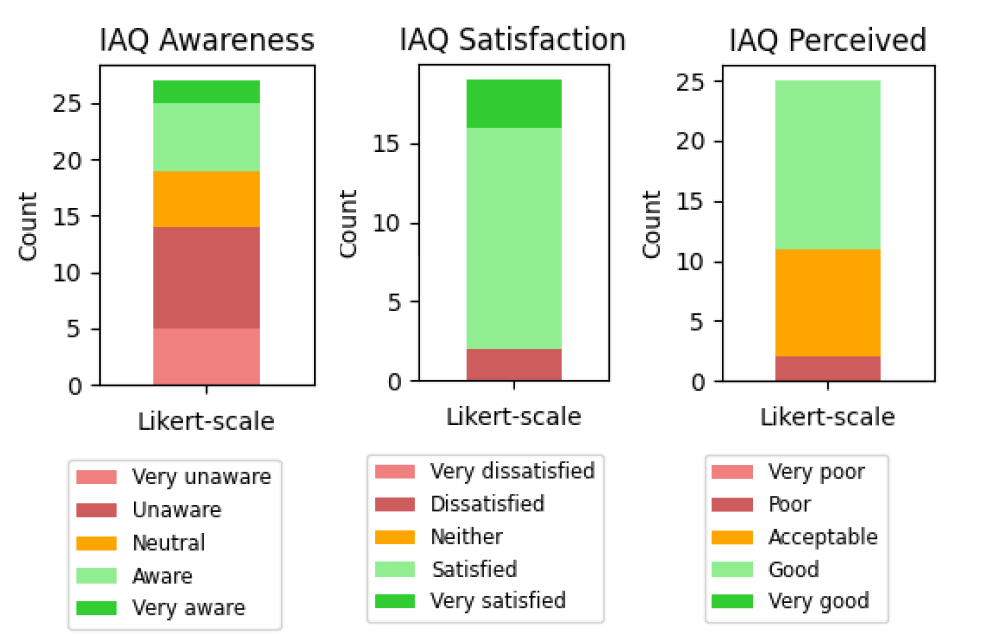
\includegraphics[width=0.5\textwidth]{IAQ_LIkert-Scales_Survey.jpg}
    \caption{Likert-scales of IAQ awareness, perception and satisfaction of the questionnaire survey with occupant count}
    \label{fig:complexity}
\end{figure}

\subsubsection{Activity and occupancy}

The first set of questions of the survey focussed on activity and occupancy. On average, occupants who filled in the survey used the Lab42 building \textit{3 times a week} for various activities ($f$=X). As opposed to 1 day a week, 4 days a week, 2 days a week with a small number of occupants using the building 5 days a week. Most occupants from the sample size were located on the \textit{ground floor ($f$=X) and the first floor ($f$=X)} as opposed to the 2nd floor. Both the first floor and ground floor are considered the 'open area' and part of the atrium of the building. This is by design of the building where the lower floors have more co-working spaces to be used as informal open learning spaces whereas the upper floors are more designed as meeting rooms and private working offices. Many occupants described the overall occupancy in the space as \textit{not too crowded} ($f$=X) with a smaller percentage explicitly stating the space was crowded or not crowded at all.

\subsubsection{Awareness, perceived and satisfaction}

The second set of questions were three Likert scales about perceived IAQ, awareness of IAQ, and satisfaction with IAQ. Over half of the occupants are \textit{not particularly aware} of the IAQ in their current space, either very unaware ($f$=X), unaware ($f$=X), or neutral ($f$=X) the minority of the occupants are aware or very aware. Indicating that in general occupants are not very aware of the IAQ if they are directly asked about it. However, once occupants are asked about their perceived IAQ and satisfaction the majority of the occupants perceive the IAQ as \textit{acceptable ($f$=X) or good ($f$=X)} and almost all occupants consider the IAQ as satisfactory by being \textit{satisfied ($f$=X) or very satisfied ($f$=X)} with the IAQ.

\subsubsection{Health and cognitive symptons}

The third set of questions were to indicate if users suffered from health or cognitive symptons based on the IAQ. The majority of participants answered \textit{none} to both the health ($f$=X) and cognitive ($f$=X) questions. A small percentage experienced health symptoms such as headaches and feeling noiziating and a larger percentage experienced cognitive symptons such as trouble with focus or tiredness. The results of this section of the survey are inconclusive since it's difficult to determine if these symptons are specifically related to the air quality.

\subsubsection{Open-ended air quality description}
The most notable finding of the open question is that the occupants who filled in the not mandatory question describing their perception of IAQ mention specifically the openness of the atrium space:

\begin{quote}
P11: "[...] think it is good, [...] although I must say that this is mostly based on the large amount of open space in the building"
\end{quote}

With some of the occupants mentioning the 'high ceilings' of the atrium specifically.

\begin{quote}
P8: " [...] feel like in this building the air quality is really good, mainly because of the impression the high ceilings give"
\end{quote}

\begin{quote}
P13: "I like the air quality. This may also be because I sit close to the door and the ceiling is high."
\end{quote}

Another notable attribute is that many occupants describe contributing to the perception that the IAQ is sufficient are the hanging planters and greenery that is present within the atrium.

\begin{quote}
P16: "[..] I also see green plants around me, of which I think they are real."
\end{quote}

\begin{quote}
P14: "[...] and the hanging plants that are present.
\end{quote}



\subsection{Air Quality Monitors}
\label{sec:monitor_analysis}

The gathered data logs are exported from the devices and analyzed with a focus on CO2 concentrations since this is the main IAQ parameter that influences air quality negatively within indoor environments. The process of breathing accumulates CO2 and the air quality within a space is heavily influenced by the occupancy within a room. Analyzation of the data logs shows occupancy patterns of a 'typical meeting', scheduled meeting patterns for the case study rooms and more notably the development of CO2 concentrations within both meeting rooms regularly where they regulary exceed optimal CO2 concentration tresholds above 600ppm.

\begin{figure}[h]
    \centering
    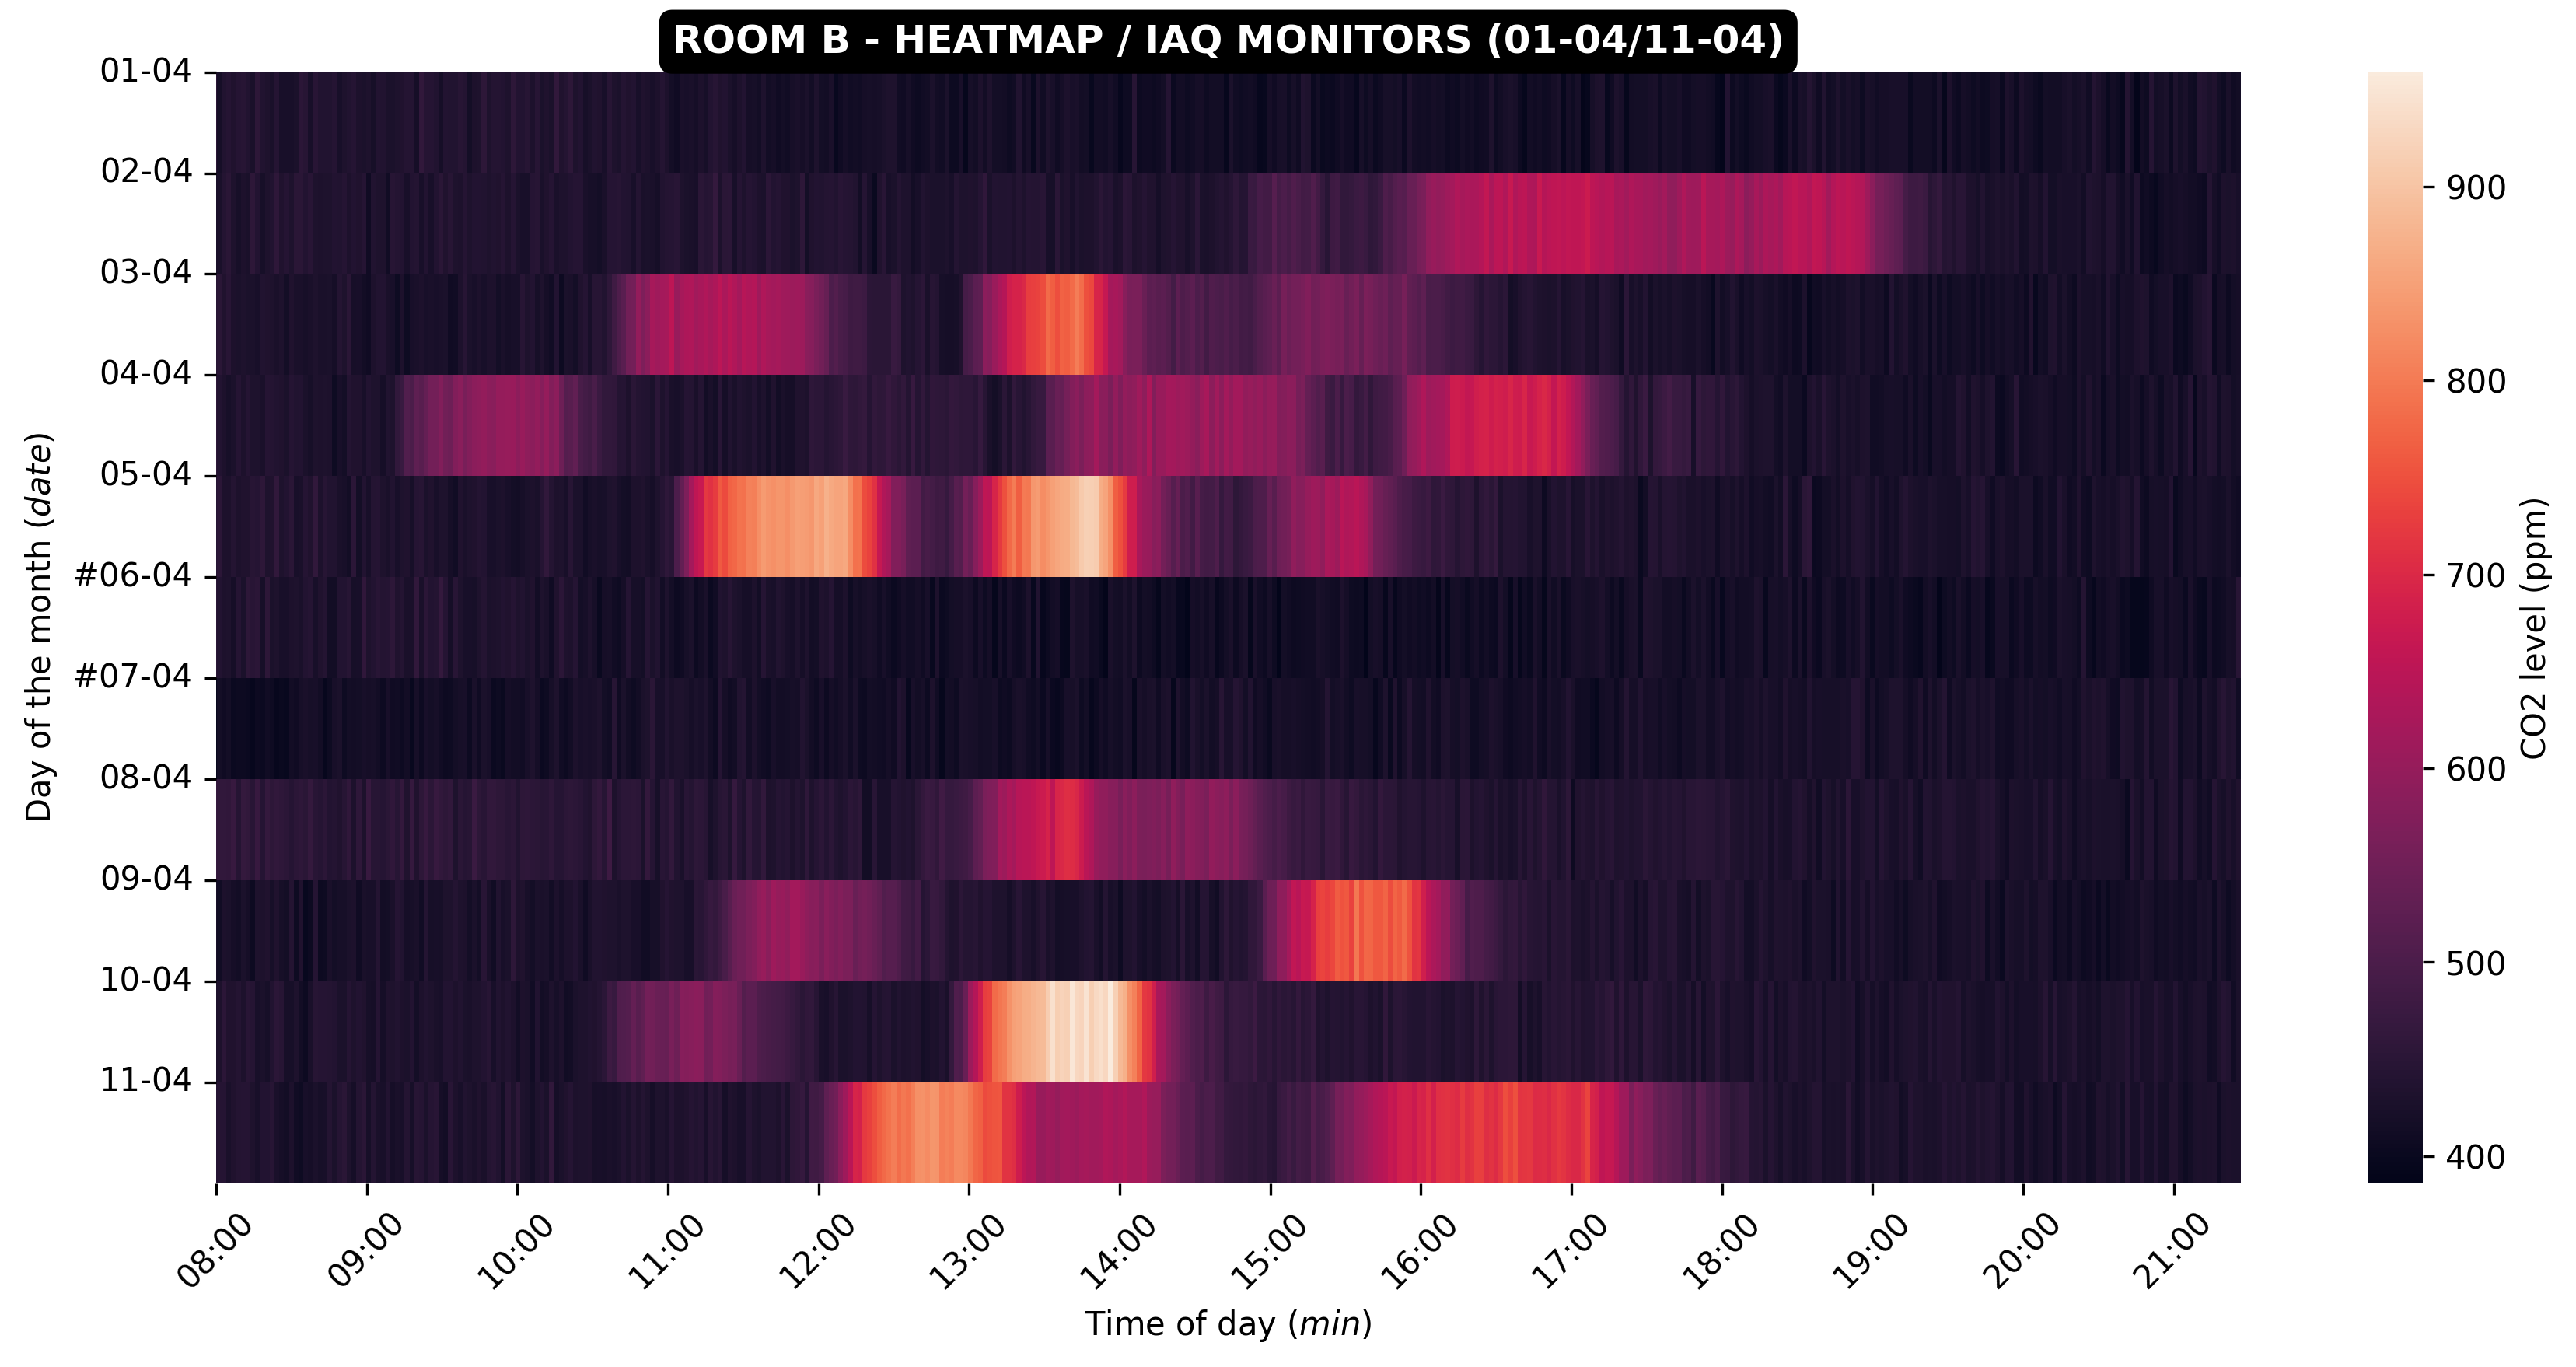
\includegraphics[width=0.5\textwidth]{room-b-monitor-heatmap.png}
    \caption{Heatmap of ten days of data logs from Room B showing the peaks of CO2 concentrations monitored }
    \label{fig:complexity}
\end{figure}

\subsubsection{Single meeting CO2 development}

A sample of CO2 concentrations in a single meeting is shown in (see \hyperref[fig:complexity]{Figure \ref*{fig:complexity}}). The lineplot shows the development of a 'regular' 1-hour meeting within the room. The plot are the CO2 concentrations over time in minutes with a x-axis line of 600ppm indicating the maximum 'ideal' treshold. Two coloured lines on the y-axis indicate the start and end time of the meeting. The observations show that after 15 minutes of the meeting started the CO2 concentrations reach suboptimal levels and continou to rise towards 950ppm level where it stabilizes as the 'maximum value' of the meeting. As stated before, continous exposure to CO2 concentrations especially between 800ppm - 1000ppm and even above are considered 'bad' and can impact cognitive functions. After ending of the meeting the concentrations slowly start to decrease to the baseline of 450ppm when occupants leave the meeting room at the end time.

\subsubsection{Regular day CO2 development}

The visualization (see \hyperref[fig:complexity]{Figure \ref*{fig:complexity}}) shows the spikes of CO2 concentrations during a sample day where multiple meetings occured. Again, the x-axis plots the CO2 concentrations and this time the y-axis shows a full day with opening hours of the building. Based on similar plots of randomly sampled days the data shows most meetings occur between late in the morning (11:00) and usually end late in the afternoon (17:00) where after no more meetings are planned. That's roughly two hours after opening of the building and roughly four hours before closing of the building. There are outliers, on some days meeting occur early in the morning straight after opening time, and occassionaly a (longer) meeting that is longer and spans longer in the evening.

\subsubsection{Meeting schedule CO2 development}

A heatmap of ten days of CO2 concentration monitoring (see \hyperref[fig:complexity]{Figure \ref*{fig:complexity}}) shows that it's common that two or three meetings occur on a single day and typically spans one hour. The majority of the meetings go beyond the 600ppm CO2 concentrations. Based on the lineplots and heatmaps it is assumed that the 'larger' Room B is more frequently used and reaches higher CO2 concentrations but those results are not definite since it heavily relies on context and the dates and time periods that spanned the data collection and the monitors were installed.

\subsection{Prototype}
\label{sec:prototype_results}

Based on the requirements, data physicalization design principles, and concept models exploration a final high fidelity (hi-fi) version of the prototype was developed that functioned as a proof-of-concept of the physical design solution as a feasibility study and utilized in the user study for evaluation.

\subsubsection{Concept description}

\textit{Bluebird} is a hanging kinetic type sculpture inspired by organic nature materials and the shapes of hanging planters that encode the environmental properties of indoor air quality data fostering the relationship with nature. It is meant to be hung from the ceiling in small to medium rooms and changes based on real-time air quality monitor data engaging the occupants within the room into considering the level of air quality. Strings (plant branches) either become longer or smaller simulating the growth of a plant. Movements of the leaves indicate the freshness of air and movement. The overall design philosophy of the shapes and forms uses the notion of calm technology to minimize interruption cost \cite{case_calm_2016}. A unique characteristic of the prototype as opposed to existing (commercially available) solutions is that it shows predictions and history, so not only feedback on the current situation when the situation of high CO2 concentrations already occurred.

\subsubsection{Electronics and components}

A controller device running on an Arduino Uno R3 \footnote{https://store.arduino.cc/products/arduino-uno-rev3} microcontroller with an MKR Motor shield is used \footnote{https://store.arduino.cc/products/arduino-motor-shield-rev3} to control six 360° MG90S type Micro Servo Motors \footnote{https://www.towerpro.com.tw/product/mg90s-3/}. Attached to these motors are pulleys with paracord rope simulating the growth of the hanging planter so that the string can be moved up and down. All electronics are integrated at the back of a wooden board, enabling the device to act as a stand-alone device making it movable and modular to be installed in other spaces.




\subsubsection{Crafting technologies and materials}
The strings, leaves, and housings of the electronics and mechanical hardware are created using additive manufacturing (3D Printing) using a Fused deposition Modeling (FDM) technique using Polylactic acid (PLA) plastic filament in various colors. The electronics enclosures and plant models were modeled using computer-aided design (CAD) software. A digital fabrication technique commonly found in data physicalization prototypes \cite{anhalt_university_germany_design_2022}. To create leaves representing textile or fabric custom properties were defined within the 3D printing software (Slicing) to remove top and bottom layers and create a thin layer of infill.

\subsubsection{System Architecture and software}

The microcontroller uses custom firmware written in Arduino code \footnote{https://www.arduino.cc/reference/en/} (similar to C++) that receives real-time data from the air quality monitors using the LoRaWAN \footnote{https://lora-alliance.org/about-lorawan/} communication protocol to control the mechanics of the prototype (see \hyperref[appendix:architecture]{Appendix \ref*{appendix:architecture}}). This arrangement of hardware is commonly found in Internet of Things (IoT) architecture set-ups and follows the notion of Edge Computing with a (1) sensing, (2) networking, (3) processing, and (4) application layer \cite{li_edge-oriented_2019, idrees_edge_2018}. Some custom library functions are written in to calculate the movements of the string. The current (\( C_{\text{current}} \) ) and previous \( C_{\text{previous}} \) CO2 concentrations are stored on which a difference number is calculated. The difference number is mapped to a movement time \( t_{\text{movement}} \) in milliseconds using a multiplication factor. Based on a negative or positive integer the servo motors spin either clockwise (growing) or counterclockwise (shrinking) the ropes.

\subsubsection{Experimental set-up}

The prototype was installed \textit{in situ} within one of the monitored meeting rooms inside of the building. We derived five relevant dimensions based on the literature; \textit{audience, intention, interaction, philosophy, representation} \cite{sauve_physecology_2022, hornecker_design_2023}.

\begin{itemize}
  \item \textbf{Audience}: visually see string become largers. Acts as a metaphor of plant 'growth'. The better the air quality the more the plant can 'grow'.
  \item \textbf{Intention}: if fresh air comes in we indicate this through movement as a metaphor for wind gusses between a field of grass or plants.
  \item \textbf{Representation}: if fresh air comes in we indicate this through movement as a metaphor for wind gusses between a field of grass or plants.
  \item \textbf{Interaction}: if fresh air comes in we indicate this through movement as a metaphor for wind gusses between a field of grass or plants.
\end{itemize}


\subsection{Evaluation}
\label{sec:evaluation_results}

The prototype-led evaluation sessions (see \ref{sec:questionnaire}) were held to assess the quality and impact of the data physicalisation with a focus on how users perceive the data embedded in the physical representation and what long-term impact it has on people.

\begin{figure}[b]
    \centering
    
\includegraphics[width=0.5\textwidth]{placeholder-two.jpg}
    \caption{Installed photograph of the prototype in the room during an evaluation session with a participant }
    \label{fig:complexity}
\end{figure}


\subsubsection{WIP (NOT FINISHED)}

Lorem Ipsum is simply dummy text of the printing and typesetting industry. Lorem Ipsum has been the industry's standard dummy text ever since the 1500s, when an unknown printer took a galley of type and scrambled it to make a type specimen book. It has survived not only five centuries, but also the leap into electronic typesetting, remaining essentially unchanged. It was popularised in the 1960s with the release of Letraset sheets containing Lorem Ipsum passages, and more recently with desktop publishing software like Aldus PageMaker including versions of Lorem Ipsum.

Lorem Ipsum is simply dummy text of the printing and typesetting industry. Lorem Ipsum has been the industry's standard dummy text ever since the 1500s, when an unknown printer took a galley of type and scrambled it to make a type specimen book. It has survived not only five centuries, but also the leap into electronic typesetting, remaining essentially unchanged. It was popularised in the 1960s with the release of Letraset sheets containing Lorem Ipsum passages, and more recently with desktop publishing software like Aldus PageMaker including versions of Lorem Ipsum.


\subsubsection{WIP (NOT FINISHED)}

Lorem Ipsum is simply dummy text of the printing and typesetting industry. Lorem Ipsum has been the industry's standard dummy text ever since the 1500s, when an unknown printer took a galley of type and scrambled it to make a type specimen book. It has survived not only five centuries, but also the leap into electronic typesetting, remaining essentially unchanged.

Lorem Ipsum is simply dummy text of the printing and typesetting industry. Lorem Ipsum has been the industry's standard dummy text ever since the 1500s, when an unknown printer took a galley of type and scrambled it to make a type specimen book. It has survived not only five centuries, but also the leap into electronic typesetting, remaining essentially unchanged Lorem Ipsum is simply dummy text of the printing and typesetting industry. Lorem Ipsum has been the industry's standard dummy text ever since the 1500s.
